The author looks at 5 years of VC \& IPO data (2011-2015) to investigate relationships b/w firm's IPO success and venture capital raised.

Dataset containing 70 'unicorns' (firms who's valuation exceeds 1B USD) was collected by Founder Collective\footnote{\url{http://www.foundercollective.com/}} VC fund, calculations by author.

See variables' description in Table \ref{tab:descr}

Facebook was excluded as an exceptinally extreme outlier.

\begin{table}[bp!]
    \centering
    \caption{Dataset variables description}
    \label{tab:descr}
    \begin{tabular}{ll}
    \textbf{Column}     & \textbf{Description}                                                   \\ \hline
    Founded             & Year the firm was founded                                              \\
    Ticker              & Firm's post-IPO stock exchange ticker                                  \\
    IPO Share Price     & Initial IPO Share Price                                                \\
    Current Share Price & Firm's share price as of Nov 22, 2016                                  \\
    Current Market Cap  & Firm's Market Cap. as of Nov 22, 2016                                  \\
    IPO Year            & Year the firm went public                                              \\
    IPO Raised          & Amount raised during the IPO (\$ mln)                                  \\
    Sector              & B2B vs B2C                                                             \\
    Geo                 & Area (State for US, City for Non-US)                                   \\
    Firm age            & Firm's age as of Nov 22, 2016                                          \\
    Years to IPO        & Years passing between firm's inception and IPO                         \\
    VC                  & Amount raised during all VC rounds (in nominal values, \$ mln)         \\
    VC and IPO          & VC Raised + IPO Raised (\$ mln)                                        \\
    \$ Price change     & Share price change from IPO to current day, as of Nov 22, 2016, in USD \\
    \% Price change     & Share price change from IPO to current day, as of Nov 22, 2016, in \%  \\
    Mult                & Multiplicator: Current Market Cap / VC Raised                         
    \end{tabular}
\end{table}


Looking at a simple bar chart plotting every single investment, we can notice that it resembles normal distribution: long tails at upper & lower values, with vast majority of observations in the middle.

\begin{figure}[ht]
    \centering
    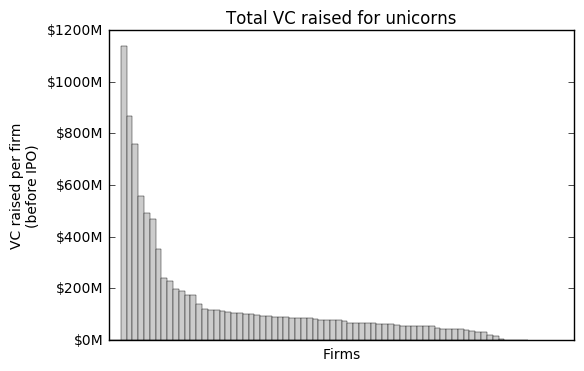
\includegraphics[scale=0.9]{vc_raised}
    \caption{ \textbf{Most funded IPOs}\\Source: Founder Collective, graph by author}
    % \label{fig:vc_raised}
\end{figure}



Table \ref{tab:b2b_b2c} compares b2b vs b2c.

Curiously, while an average B2B startup has significantly less funding (56\% less) than a B2C one, it's average valuation is only 15\% lower.

This is most probably due to the fact that startups in B2C field face stiffer competition, have to attract new users, and may not have a robust monetization model for a long time.

At the same time, B2B due to it's business-oriented nature often starts generating cash at early stages.


\begin{table}[bp!]
    \centering
    \begin{tabular}{lcc}
        \toprule
         &      VC & Current Market Cap \\
        \midrule
        B2C Total   &  \$6,053 &            \$96,775 \\
        B2B Total   &  \$3,550 &           \$111,356 \\
        B2C Average &    \$201 &             \$3,225 \\
        B2B Average &     \$88 &             \$2,783 \\
        \bottomrule
    \end{tabular}
    \caption{B2B vs B2C Comparison, author's calculations from dataset}
    \label{tab:b2b_b2c}
\end{table}


Now let's compare 20 most vs 20 least funded startups: the less funded ones, according to Multiplicator, are on average 5 times more efficient.

It's an interesting finding, since some would expect a contrary result, where more money creates more business opportunities and higher efficiencies. Apparently, it is not the case, and the investors should beware of over-pumping the startup with easy money.

The challenge is to find a funding balance which will cover all necessary business and R\&D costs while keeping the team 'hungry' and 'nimble'.

\begin{table}
    \centering
    \begin{tabular}{lccc}
    \toprule
    {} &      VC &  Current Market Cap &   Mult \\
    \midrule
    most\_20  &  332.69 &             3182.94 &  12.96 \\
    least\_20 &   44.91 &             2183.98 &  63.04 \\
    \bottomrule
    \end{tabular}
\end{table}

%%%%%%%%%%%%%%%%%%%%%%%%%%%%%%%%%
%%%%%     first OLS result %%%%%%
%%%%%%%%%%%%%%%%%%%%%%%%%%%%%%%%%
Evaluating coefficients of regression is performed on the basis of OLS (Ordinary Least Squares), using StatsModels \footnote{\url{http://www.statsmodels.org/}} package for Python \footnote{\url{http://www.python.org/}}

\vspace{0.1cm}

\begin{center}
    \begin{tabular}{lclc}
    \toprule
    \textbf{Dep. Variable:}    &      Growth      & \textbf{  R-squared:         } &     0.137   \\
    \textbf{Model:}            &       OLS        & \textbf{  Adj. R-squared:    } &     0.084   \\
    \textbf{Method:}           &  Least Squares   & \textbf{  F-statistic:       } &     2.577   \\
    \textbf{Date:}             & Tue, 21 Nov 2016 & \textbf{  Prob (F-statistic):} &   0.0456    \\
    \textbf{Time:}             &     10:39:48     & \textbf{  Log-Likelihood:    } &   -103.41   \\
    \textbf{No. Observations:} &          70      & \textbf{  AIC:               } &     216.8   \\
    \textbf{Df Residuals:}     &          65      & \textbf{  BIC:               } &     228.1   \\
    \textbf{Df Model:}         &           4      & \textbf{                     } &             \\
    \bottomrule
    \end{tabular}
    \begin{tabular}{lccccc}
                              & \textbf{coef} & \textbf{std err} & \textbf{t} & \textbf{P$>$$|$t$|$} & \textbf{[95.0\% Conf. Int.]}  \\
    \midrule
    \textbf{Intercept}        &       0.4750  &        0.725     &     0.655  &         0.515        &        -0.974     1.924       \\
    \textbf{C(Sector)[T.B2C]} &      -0.3221  &        0.284     &    -1.132  &         0.262        &        -0.890     0.246       \\
    \textbf{VC}               &      -0.0015  &        0.001     &    -2.124  &         0.037        &        -0.003 -9.22e-05       \\
    \textbf{Age}              &       0.2197  &        0.109     &     2.022  &         0.047        &         0.003     0.437       \\
    \textbf{yearsIPO}         &      -0.2489  &        0.109     &    -2.283  &         0.026        &        -0.467    -0.031       \\
    \bottomrule
    \end{tabular}
    \begin{tabular}{lclc}
    \textbf{Omnibus:}       &  4.643 & \textbf{  Durbin-Watson:     } &    2.150  \\
    \textbf{Prob(Omnibus):} &  0.098 & \textbf{  Jarque-Bera (JB):  } &    4.076  \\
    \textbf{Skew:}          &  0.586 & \textbf{  Prob(JB):          } &    0.130  \\
    \textbf{Kurtosis:}      &  3.152 & \textbf{  Cond. No.          } & 1.34e+03  \\
    \bottomrule
    \end{tabular}
    %\caption{OLS Regression Results}
\end{center}


The OLS model \ref{eq:OLS_hat} has $Prob(F-statistic) < 0.05$, so at $\alpha = 5\%$ it is statistically significant as a whole.

Interestingly, $VC$ is significant has coeff of $-0.0015$. It is counter-intuitive that increasing investment in a firm can have negative effect on it's rate of share growth.

One possible explanation is that during an IPO.  well-funded successfull firms are priced more optimistically than their less inflated counterparts. Then over the years firms with lower initial valuation find it easier to grow in value faster.

While $Age$ and $yearsIPO$ are obviously correlated , removing one or the other degrades the model's accuracy to the point where it becomes invalid at $\alpha = 5\%$.